\documentclass[12pt]{article}
\usepackage{hyperref}
\usepackage{listings}
\usepackage{biblatex}
\usepackage{tikz}
\usepackage{refstyle}
\usepackage{mathabx}
\usepackage{amssymb}
\usepackage{caption}
\usepackage{float}
\usepackage{graphicx}
\usepackage{graphics}
\usepackage{subfig}

\graphicspath{{/storage/self/primary/Download/latexnew/fig}}
\begin{document}
\title{\textbf{PLATFORMIO}}
\date{}
\maketitle
\begin{enumerate}
    \item \textbf{Question(GATE-EC-2018-31):}A four-variable Boolean function is realized using $4\times 1$ multiplexers as shown in the 
    \begin{figure}[!h]
        \centering
        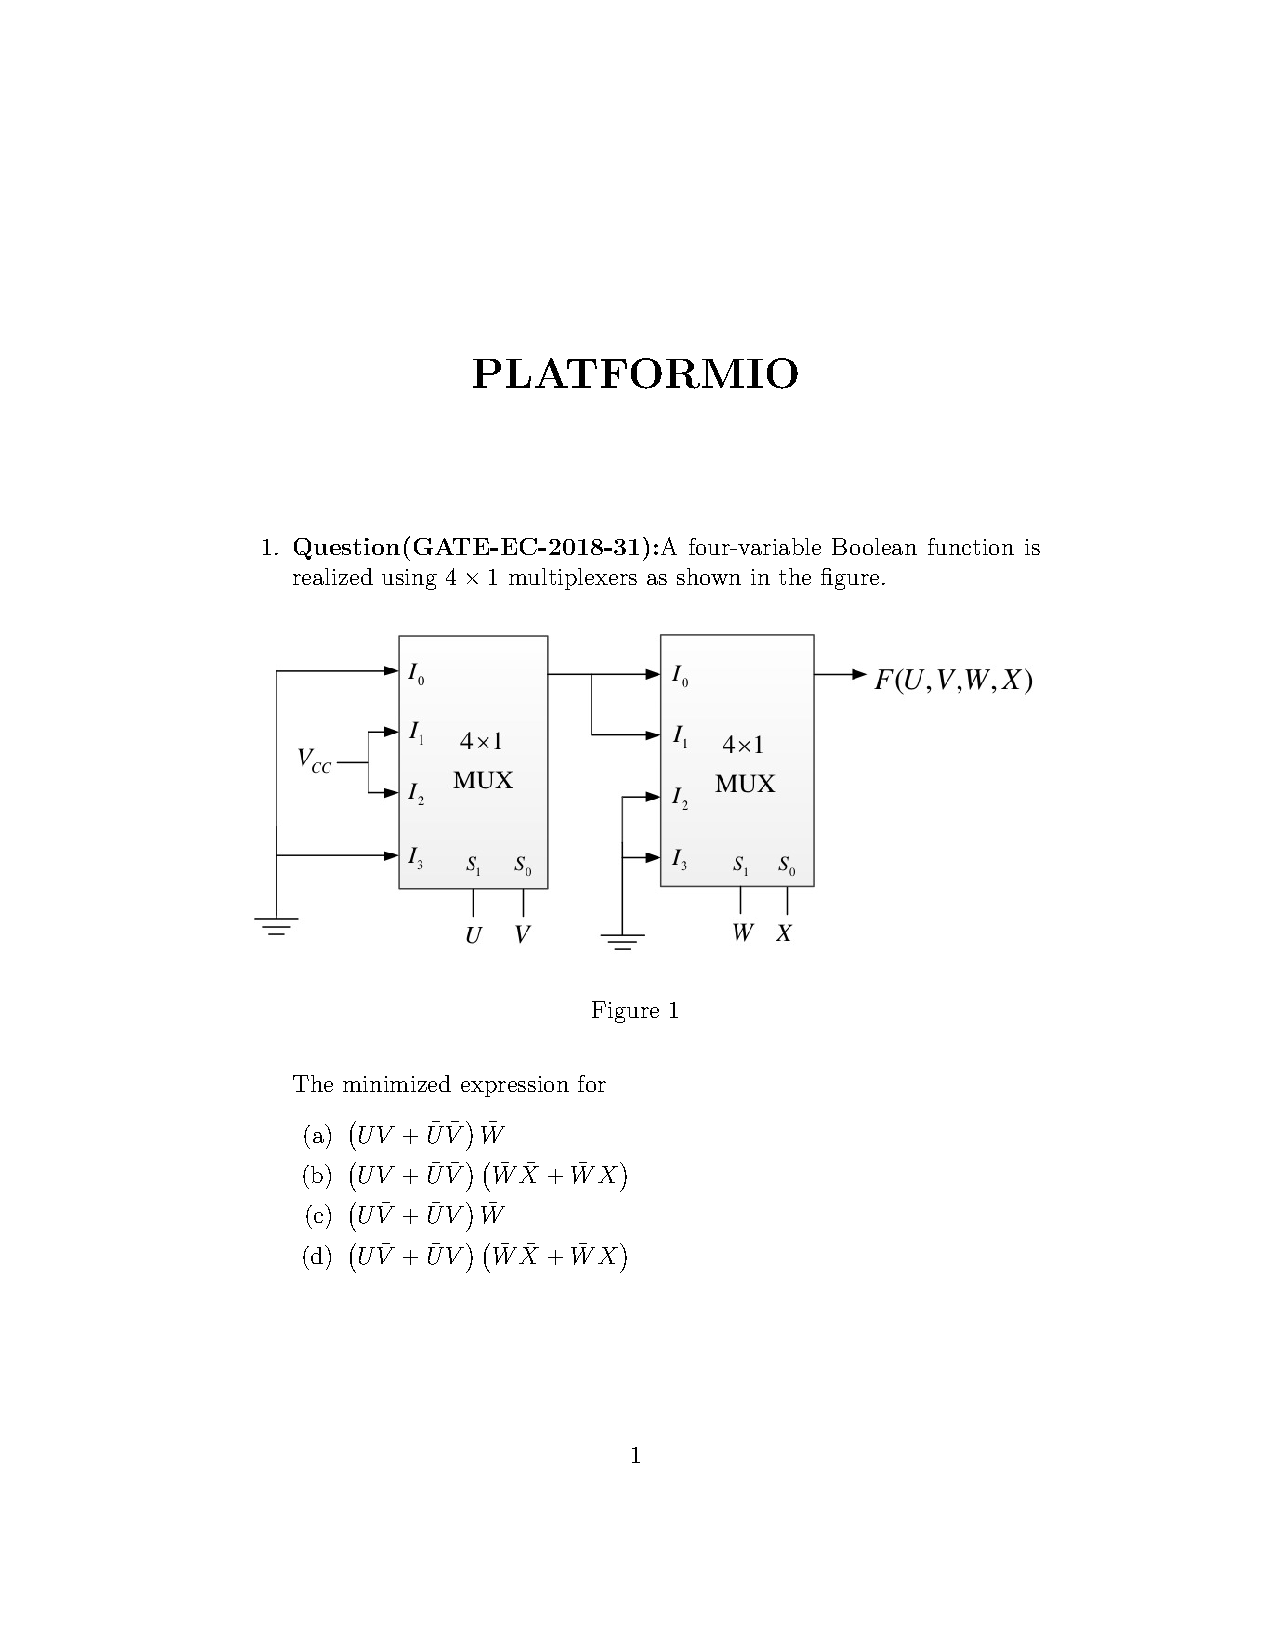
\includegraphics[width=\columnwidth]{mux.png}
        \caption{Logic realised by the circuit shown in figure}
        \label{fig:mux}
    \end{figure}

   The minimized expression for 
    \begin{enumerate}
       \item $\left ( UV+\bar{U}\bar{V} \right )\bar{W}$
       \item $\left ( UV+\bar{U}\bar{V} \right )\left ( \bar{W}\bar{X}+\bar{W}X\right )$
       \item $\left ( U\bar{V}+\bar{U}V \right )\bar{W}$
       \item $\left ( U\bar{V}+\bar{U}V \right )\left ( \bar{W}\bar{X}+\bar{W}X\right )$
    \end{enumerate}


\end{enumerate}


\end{document}
